\section{Problem Framework}

\begin{frame}{Anomaly Detection in Satellite Telemetry}
   \begin{center}
      \Large\textcolor{BrickRed}{\textbf{Context}}

      \vspace{0.25cm}

      \small{Satellites generate \underline{continuous multi-channel time-series telemetry} to monitor system health}
   \end{center}

   \pause
   \vfill

   \begin{center}
      \Large\textcolor{BrickRed}{\textbf{Problem}}

      \vspace{0.25cm}

      \small{\underline{Anomalies} can occur, leading to critical system failures and loss of spacecraft functionality}
   \end{center}

   \pause
   \vfill

   \begin{center}
      \Large\textcolor{BrickRed}{\textbf{Idea}}

      \vspace{0.25cm}

      \small{Employ a neural network model to automate \underline{time-series anomaly detection}}
   \end{center}
\end{frame}

\subsection{OPS-SAT Dataset}

\begin{frame}{ESA Telemetry Benchmark}
   \small{Our reference is \underline{real in-orbit operational time-series} data provided by ESA}

   \pause
   \vfill

   \begin{minipage}[c]{0.33\textwidth}
      \textbf{OPS-SAT CubeSat}
   \end{minipage}
   \begin{minipage}[c]{0.65\textwidth}
      \footnotesize
      $\left\{ 
         \begin{array}{l}
            \textbf{303,493} \text{ temporal points}\\
            \textbf{2,123} \text{ continuous segments}\\
            \textbf{9} \text{ telemetry sensors}\\
            \textbf{1\,s} \text{ median sampling interval } (\Delta t)\\
            \text{Labels: } \sim\textbf{80\%} \text{ nominal, } \sim\textbf{20\%} \text{ anomalous}\\
         \end{array}
      \right.$
      \normalsize
   \end{minipage}

   \pause
   \vfill

   Originally designed for unsupervised anomaly detection in a reconstruction framework, the task is framed here as a \textcolor{BrickRed}{\textbf{supervised binary classification}} problem suited for a simpler model architecture
\end{frame}

\begin{frame}{Telemetry example}

   Slice of a continous telemetry segment that shows \textbf{quasi-periodic oscillations}. Anomalies are highlighted in red, displaying strong deviations from the normal signal.

   \vfill

   \begin{center}
      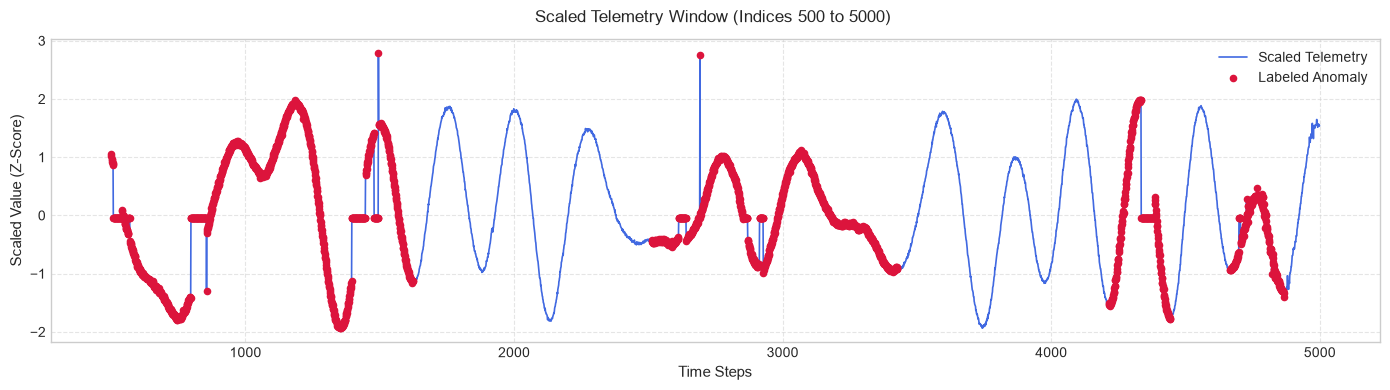
\includegraphics[width=\textwidth]{Immagini/telemetry-example.png}
   \end{center}
\end{frame}

\begin{frame}[t]{Preprocessing Pipeline}
   Key data preparation steps tailored for our classification framework:

   \vspace{0.4cm}

   \begin{overlayarea}{\linewidth}{5.8cm}
      \only<1>{
         \begin{itemize}
            \item \large{\textbf{Data splitting}}
            
            \normalsize{Split between training, validation and test sets at the segment level prior to further processing to prevent overlapping sequence leakage across sets.}
         \end{itemize}
      }

      \only<2>{
         \begin{itemize}
            \item \large{\textbf{Channel-wise normalization}}
            
            \normalsize{Standardize each sensor independently using empirical mean $\mu$ and standard deviation $\sigma$ estimated on nominal training data to avoid data leakage.}
         \end{itemize}

         \vspace{0.3cm}
         \begin{center}
            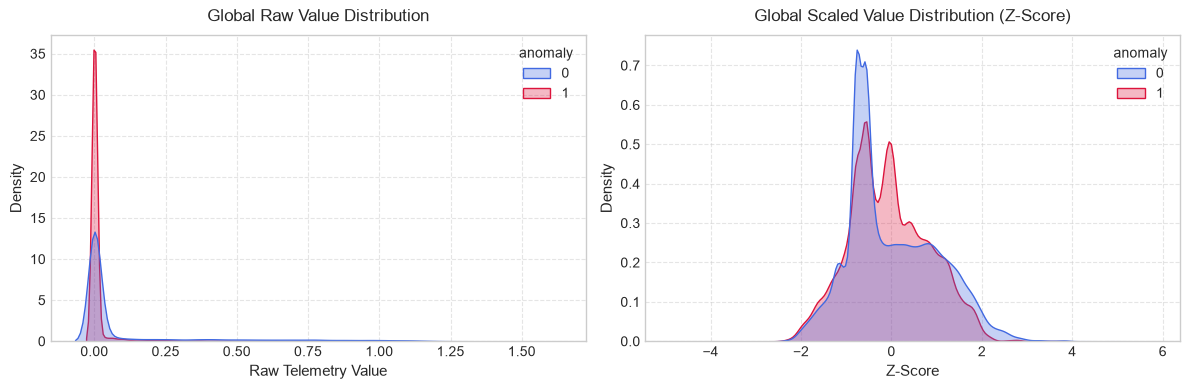
\includegraphics[width=\linewidth]{Immagini/data-normalization.png}
         \end{center}
      }

      \only<3>{
         \begin{itemize}
            \item \large{\textbf{Sliding window}}
            
            \normalsize{Extract fixed-length ($W=50$) temporal windows within segments, mapping sequence $(x_{t-49},\dots,x_t)$ to target label $y_t \in \{0, 1\}$ with stride $S=5$ for training (to reduce redundancy) and $S=1$ for validation and test}
         \end{itemize}

         \vspace{0.3cm}
         \begin{center}
    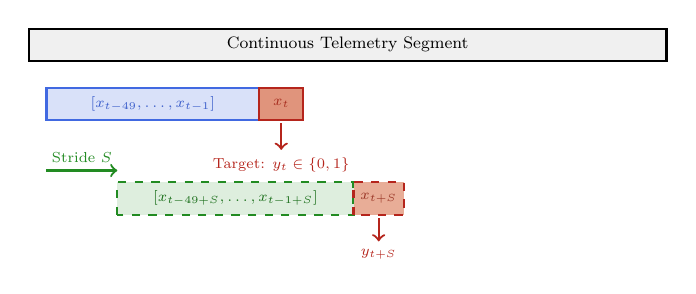
\begin{tikzpicture}[scale=0.75, every node/.style={transform shape}]
        \draw[thick, fill=gray!12] (0, 0) rectangle (10.8, 0.55);
        \node at (5.4, 0.28) {\footnotesize Continuous Telemetry Segment};

        \draw[thick, RoyalBlue, fill=RoyalBlue!20] (0.3, -1.0) rectangle (3.9, -0.45);
        \draw[thick, BrickRed, fill=BrickRed!40] (3.9, -1.0) rectangle (4.65, -0.45);
        \node[RoyalBlue!90!black] at (2.1, -0.72) {\scriptsize $[x_{t-49}, \dots, x_{t-1}]$};
        \node[BrickRed!90!black] at (4.275, -0.72) {\scriptsize $x_t$};
        
        \draw[->, thick, BrickRed] (4.275, -1.05) -- (4.275, -1.5) node[below] {\scriptsize Target: $y_t \in \{0, 1\}$};

        \draw[->, thick, ForestGreen] (0.3, -1.85) -- (1.5, -1.85) node[midway, above] {\scriptsize Stride $S$};

        \draw[thick, dashed, ForestGreen, fill=ForestGreen!15] (1.5, -2.6) rectangle (5.5, -2.05);
        \draw[thick, dashed, BrickRed, fill=BrickRed!30] (5.5, -2.6) rectangle (6.35, -2.05);
        \node[ForestGreen!80!black] at (3.5, -2.32) {\scriptsize $[x_{t-49+S}, \dots, x_{t-1+S}]$};
        \node[BrickRed!80!black] at (5.925, -2.32) {\scriptsize $x_{t+S}$};
        \draw[->, thick, BrickRed] (5.925, -2.65) -- (5.925, -3.05) node[below] {\scriptsize $y_{t+S}$};
    \end{tikzpicture}
\end{center}
      }
   \end{overlayarea}
\end{frame}

\subsection{Neural Network Architecture}

\subsection{Training Performance}